%%%%%%%%%%%%%%%%%%%%%%%%%%%%%%%%%%%%%%%%%%%%%%%%%%%%%%%%%%%%%%%%%%%%%%%%%%%%%%%%
%2345678901234567890123456789012345678901234567890123456789012345678901234567890
%        1         2         3         4         5         6         7         8

\documentclass[letterpaper, 10 pt, conference]{ieeeconf}  % Comment this line out
                                                          % if you need a4paper
%\documentclass[a4paper, 10pt, conference]{ieeeconf}      % Use this line for a4
                                                          % paper

\IEEEoverridecommandlockouts                              % This command is only
                                                          % needed if you want to
                                                          % use the \thanks command
\overrideIEEEmargins
% See the \addtolength command later in the file to balance the column lengths
% on the last page of the document



% The following packages can be found on http:\\www.ctan.org
\usepackage{amsmath} % assumes amsmath package installed
\usepackage{amssymb}  % assumes amsmath package installed
\usepackage{tikz} % assumes tikz package installed
\usepackage{subfig} % assumes subfig package installed
\title{\LARGE \bf
Inferring Network Topology from Chaotic Time Series
}

\author{Parker King-Fournier \\
		parker.king-fournier "at" gmail.com}

\begin{document}

\maketitle
\thispagestyle{empty}
\pagestyle{empty}

%%%%%%%%%%%%%%%%%%%%%%%%%%%%%%%%%%%%%%%%%%%%%%%%%%%%%%%%%%%%%%%%%%%%%%%%%%%%%%%%
\begin{abstract}
Significant interest has been shown in the ability of ecologic networks to generate chaotic dynamics: it has been shown that simple ecologic models can generate dynamics that neither reach an equilibrium nor a stable limit cycle but oscillate around a strange attractor. As a result, the dynamics of ecologic networks has proved challenging to analyze using traditional ecologic techniques. Recently, machine learning has been shown to be quite effective in the areas of classification, regression and forecasting of time series, both chaotic and not. In this paper three different machine learning models are used to classify and regress time series resulting from ecologic models that have been found to exhibit chaotic behavior. Specifically, a Deep Neural Network (DNN), Convolutional Neural Network (CNN) and a Convolutional - Long Short-Term Memory Network (CNN-LSTM) are used to classify which ecologic network generated a given time series, and to regress three different topologic metrics (the connectance, characteristic path length, and links per species) of the ecologic network that generated that time series. In comparing these machine learning models, a positive correlation between model complexity and model performance was found, with the CNN-LSTM performing on average best, the CNN second best, and the DNN worst.
\end{abstract}
\begin{keywords}
chaos theory, chaotic attractors, convolutional neural networks, deep neural networks, dynamical systems, ecology, food webs, long short-term memory, machine learning, network topology, sequence classification, regression, time series 
\end{keywords}


%%%%%%%%%%%%%%%%%%%%%%%%%%%%%%%%%%%%%%%%%%%%%%%%%%%%%%%%%%%%%%%%%%%%%%%%%%%%%%%%
\section{INTRODUCTION}
	Chaos Theory has provided explanations to the seemingly unpredictable nature of many systems in our universe. Characterized by their sensitivity to initial conditions, chaotic systems yield drastically different results from minute changes in starting conditions, making them difficult to analyze using traditional methods. Systems both natural and man-made have been shown to exhibit chaotic behavior. In nature chaos is found often in the flow of liquid and gases. The famous Lorenz system, a simplified model of atmospheric weather patterns, shows chaotic dynamics for certain parameter settings (Lorenz, 1993). Man-made systems, such as the double pendulum and logistic map have helped further the understanding of chaos and its applications.

	The study of chaos has been widely successful to the study of time series (Liu, 2010), showing how markets, particles' positions, or populations may change over time. In the field of ecology the well known Lynx-Hare Cycle has shown that population dynamics of species may be governed by chaos (Maquet, 2007). The application of chaos theory to the study of population dynamics has continued and, has been successful in describing the populations of species contained within certain food web structures (Klebanoff, 1994).

	Due to the deterministic nature of chaos, a chaotic system can be successfully predicted if the underlying processes of the system are known. Without this information however, the prediction and overall analysis of these systems is difficult due to the erratic characteristics present. Recent developments in the field of Machine Learning have increased the ability to predict and characterize chaotic systems. Because these algorithms have the ability to learn complex functions, extract features from data and generalize well, Machine Learning is being used to explore chaotic systems in both academia and industry. 
    
	Despite the rising popularity of Machine Learning, its use in the field of ecology has been slow growing. The presence of chaos in ecology and the ability for Machine Learning to understand complicated dynamics exposes one use of Machine Learning in ecology and is the main motivation for the following report.
    
    Below is a detailed description of one such application of the power Machine Learning in the analysis of chaotic dynamics originating from ecological systems. First, datasets of population data were created from food web models which are known to show chaos. Each point in these datasets contain are of the form \textit{(x,y)} with \textit{x} being chaotic population time series, and \textit{y} being a labelling related to the ecologic network that generated time series \textit{x}. Datasets labelled with topologic metrics are used for regression, whereas datasets with labels of which ecologic network generated a time series are used for classification. For the specific task of classification, the original dataset was split into smaller data-subsets to compare machine learning model performance between these subsets. 

    These datasets are then used to train three machine learning algorithms with the aim of a) classifying the population time series by identifying the food web topology that generated a given time series and b) regressing the value of a topologic metric of the food web that generated a time series. The results are given, then interpreted with respect to their importance in the fields of deep learning, topology and ecology, and improvements to the models and datasets are discussed so that further research may be well directed.


%%%%%%%%%%%%%%%%%%%%%%%%%%%%%%%%%%%%%%%%%%%%%%%%%%%%%%%%%%%%%%%%%%%%%%%%%%%%%%%%
\section{RELATED WORK}
	As stated above, the presence of chaos in ecologic systems has been the focus of much previous research. In \textit{"Do Strange Attractors Govern Ecological Systems?"} Schaffer and Kot explored the presence of chaotic dynamics in theoretical models as well as real world data (Schaffer \& Kot, 1985). The chaos was visualized revealing attractors along which various natural systems travel. Schaffer and Kot challenged the existing understanding of natural systems, speculating that (then) current linear models may severely misrepresent the complexity of nature. 
    
	Furthermore, the authors speculated that natural systems may be entirely nonlinear saying, "Our own opinion is that what passes for fundamental concepts in ecology is as mist before the fury of the storm-in this case, a full, nonlinear storm" (Schaffer \& Kot, 1985). Although significant time has passed since publication, this work provides important theoretic and empirical evidence that chaos is present in natural systems. 
    
	It is well established that food webs can generate chaotic dynamics for certain parameter settings. In 1994 Aaron Klebanoff and Alan Hastings showed chaotic dynamics in their paper titled \textit{"Chaos in one-predator, two-prey models: General results from bifurcation theory"} (Klenaboff \& Hastings, 1994). Their work showed that a relatively simple system can produce extremely erratic results, and again secured the place of Chaos Theory in ecology. 
  
	The prospect of inferring network topology from data is an important problem in ecology. Previous work includes the inference of topology in spatial networks (Barthelemy et al., 2010), as well as the inference of topology in networks describing species interaction (Vera-Licona \&  Laubenbacher, 2008). 
  
	In \textit{"Inferring topology from dynamics in spatial networks"}, Gilarranz et al. attempted to discern the degree to which the dynamical patterns reveal underlying dispersal pathways. Their attempt was unsuccessful but their apparent failure proved to be helpful by showing that further constraints must be made in order to make the inference more manageable for our current technologies. This was a main factor in the decision to restrict the number of classes present in the datasets created for this report. 

	The classification of population data into different generating topologies falls under the larger task of sequence classification. In the Machine Learning community sequence classification has been used in a variety of applications, from medical diagnosis to human-robot differentiation (Dietterich, 2002). Of particular interest is the recent work on the performance of Deep Learning methods, specifically Long Short Term Memory (LSTMs) Networks, in sequence classification. In 2005 Alex Graves and Jurgen Schmidhuber found that LSTM Networks outperformed traditional Recurrent Neural Networks (RNNs) and Multilayer Perceptrons (MLPs) in speech processing. While speech processing may seem a long way from ecological networks, the performance of the networks in the task of sequence classification inspired some of the architectures used below. 

%%%%%%%%%%%%%%%%%%%%%%%%%%%%%%%%%%%%%%%%%%%%%%%%%%%%%%%%%%%%%%%%%%%%%%%%%%%%%%%%
\section{PROBLEM DESCRIPTION}
\begin{figure}
  \centering
  \subfloat[The ZYX phase space]{\label{ref_label1}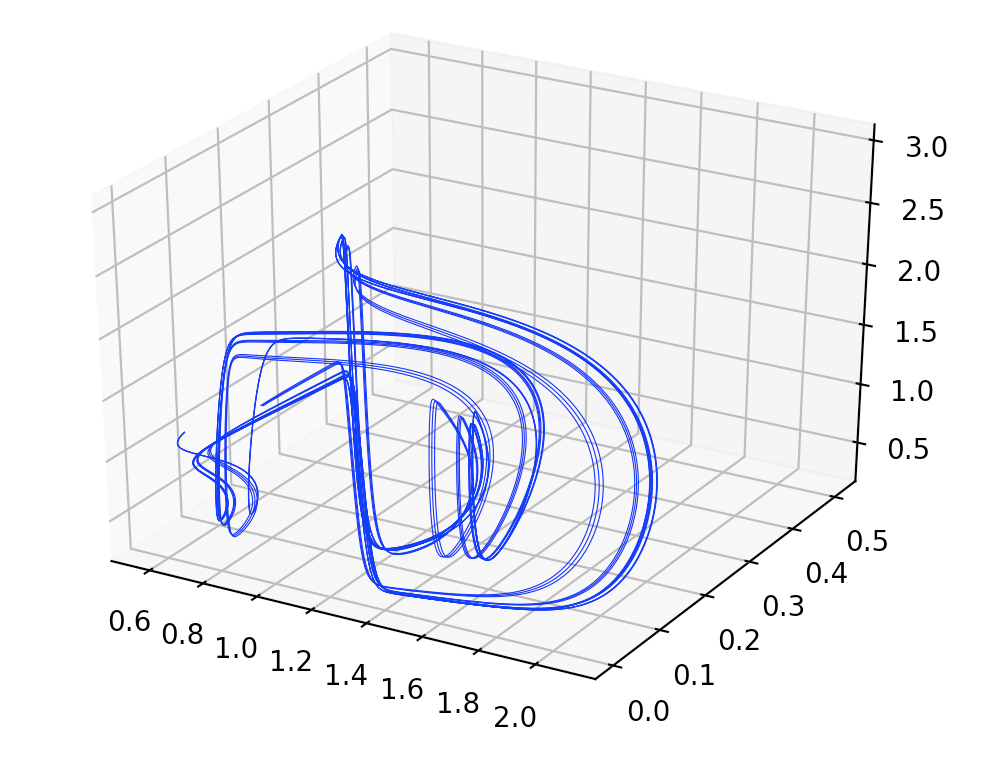
\includegraphics[width=0.5\textwidth]{zyx.png}}\\
  \subfloat[The ZYP phase space]{\label{ref_label2}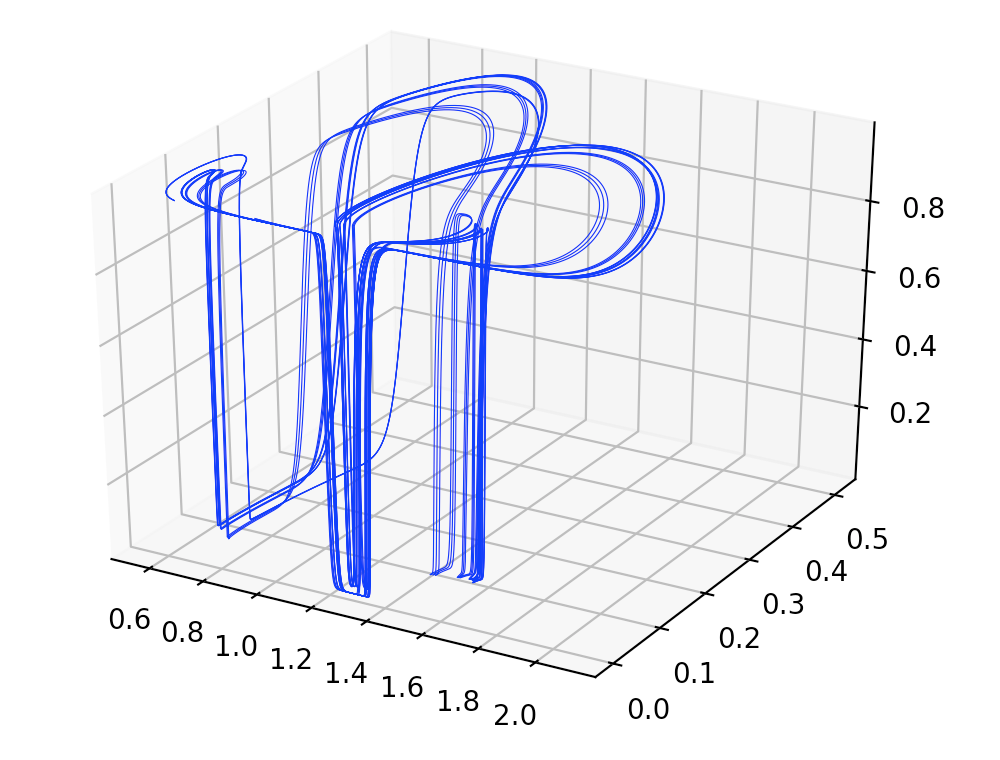
\includegraphics[width=0.5\textwidth]{zyp.png}}\\
  \subfloat[The YXC phase space]{\label{ref_label3}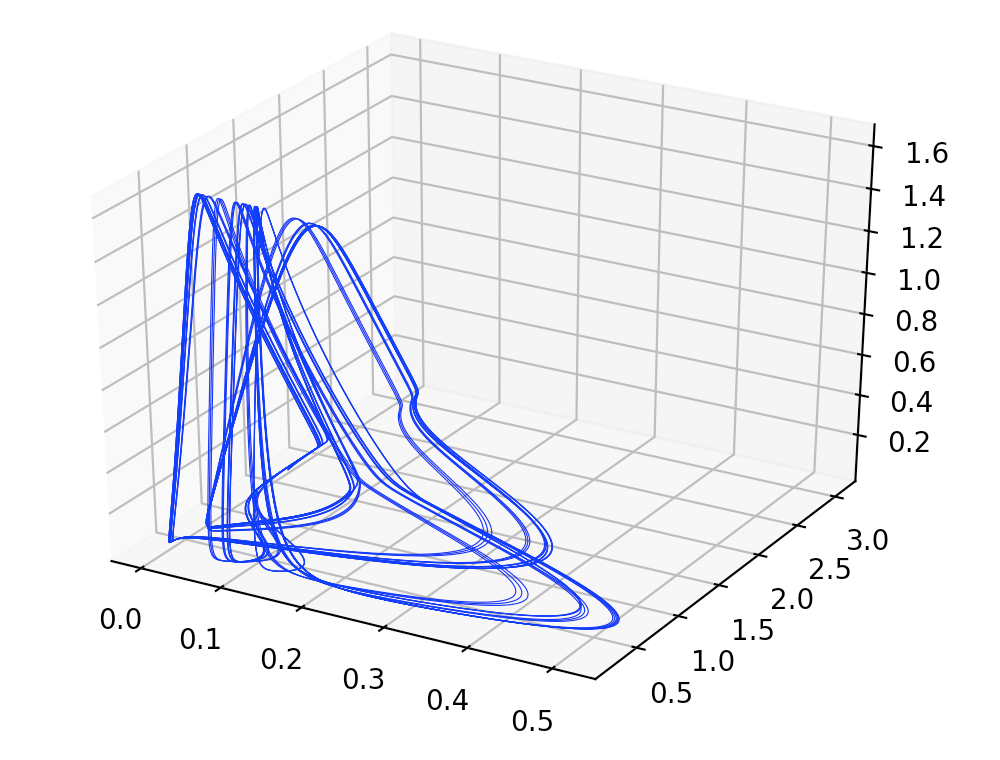
\includegraphics[width=0.5\textwidth]{yxc.png}}\\
  \caption{\label{ref_label_overall}3 phase space trajectories of a 5 species chain with parameters \textit{d\textsubscript{Z}} = 0.01, \textit{d\textsubscript{Y}} = 0.01, \textit{d\textsubscript{X}} = 0.01 and \textit{d\textsubscript{C}} = 0.11. The trajectories start with all species at 0.5, 0.500037 and 0.500075, respectively, and were evaluated for 220,000 time steps, omitting the first 60,000. Z represents the apex predator of the chain, Y is predated by Z, X is predated by Y, C is predated by X and P is predated by C.}
\end{figure}
    The goal of the research presented was to attempt to infer characteristics of the underlying food web topology of a system given a population single time series. Originally the aim was to generate the underlying topology after observing a time series, however it became clear early on that this approach was too broad. To narrow the scope the number of topologies considered was limited to eight different network structures and the task was redefined to a) classify the topology that generated a time series and b) regress a topologic metric of the topology that generated a time series. 
    
    Preexisting ecologic network topologies were used to generate chaotic time series that were stored in a datasets containing points of the form \textit{(X , Y)}, where \textit{X} is the time series of a single species and Y is either the food web topology that generated \textit{X}, or the a topologic metric of the food web topology that generated \textit{X}. To further understand the difference between topologies, the dataset containing labels corresponding to network topologies was relabeled and stored into a new data set of the form \textit{(X , Y’)}, where \textit{X} remains unchanged and \textit{Y} is the number of species in the topology that generated \textit{X}. From this dataset, three more datasets were constructed, each containing time series generated from topologies that all contain the same number of species. These sets were stored in the same format as the previously mentioned datasets. It is paramount to understand these datasets and their relation to one another. Because they may be somewhat confusing, a more rigorous description of the datasets is below.

    
    After creating the datasets, three classification algorithms were trained on each data set, and the highest accuracy for each were recorded. The classification algorithms used represented a variety of approaches to classification: specifically these algorithms were a Deep Neural Network (DNN), Convolutional Neural Network (CNN), and a Convolutional - Long Short Term Memory Network (CNN-LSTM). 
    
\subsection{Ecological Models}
\begin{table}
\tikzstyle{every node}=[circle, draw, fill=black,
                        inner sep=0pt, minimum width=1pt]
\caption{Food Web Topologies}
\setlength{\tabcolsep}{5mm} % separator between columns
\def\arraystretch{1.25} % vertical stretch factor
\centering

  \begin{tabular}{|c|c|c|}
	\hline
    & A & B \\
    \hline
    1 & 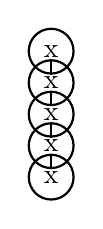
\begin{tikzpicture}[thick,scale=0.8]
   		\node at (0,-0) [circle,draw] (a) {x};
        \node at (0,-0.5) [circle,draw] (b) {x};
        \node at (0,-1) [circle,draw] (c) {x};
        \node at (0,-1.5) [circle,draw] (d) {x};
        \node at (0,-2) [circle,draw] (e) {x};
        \draw (a) -- (b) -- (c) -- (d) -- (e);
    \end{tikzpicture} &
    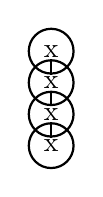
\begin{tikzpicture}[thick,scale=0.8]
   		\node at (0,0) [circle,draw] (a) {x};
        \node at (0,-0.5) [circle,draw] (b) {x};
        \node at (0,-1) [circle,draw] (c) {x};
        \node at (0,-1.5) [circle,draw] (d) {x};
        \draw (a) -- (b) -- (c) -- (d);
    \end{tikzpicture} \\  
    \hline
    
    2 & 
    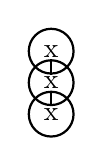
\begin{tikzpicture}[thick,scale=0.8]
   		\node at (0,0) [circle,draw] (a) {x};
        \node at (0,-0.5) [circle,draw] (b) {x};
        \node at (0,-1) [circle,draw] (c) {x};
        \draw (a) -- (b) -- (c);
    \end{tikzpicture} &
    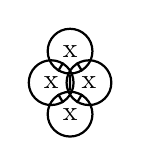
\begin{tikzpicture}[thick,scale=0.8]
   		\node at (0,0) [circle,draw] (a) {x};
        \node at (-0.3,-0.5) [circle,draw] (b1) {x};
        \node at (0.3,-0.5) [circle,draw] (b2) {x};
        \node at (0,-1) [circle,draw] (c) {x};
        \draw (a) -- (b1) -- (c) (a) -- (c) (a) -- (b2) -- (c);
    \end{tikzpicture}  \\ 
    \hline
    
    3 & 
    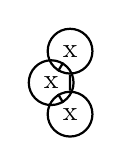
\begin{tikzpicture}[thick,scale=0.8]
   		\node at (0,0) [circle,draw] (a) {x};
        \node at (-0.3,-0.5) [circle,draw] (b) {x};
        \node at (0,-1) [circle,draw] (c) {x};
        \draw (a) -- (b) -- (c) (a) -- (c);
    \end{tikzpicture}   &
    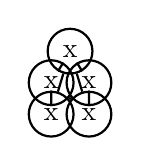
\begin{tikzpicture}[thick,scale=0.8]
   		\node at (0,0) [circle,draw] (a) {x};
       	\node at (-0.3,-0.5) [circle,draw] (b1) {x};
        \node at (0.3,-0.5) [circle,draw] (b2) {x};
        \node at (-0.3,-1) [circle,draw] (c1) {x};
        \node at (0.3,-1) [circle,draw] (c2) {x};
        \draw (a) -- (b1) -- (c1) (a) -- (b2) -- (c2) (b1) -- (c2) (b2) -- (c1) (a) -- (c1) (a) -- (c2);
    \end{tikzpicture} \\ 
    \hline
   
   4 & 
   	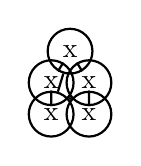
\begin{tikzpicture}[thick,scale=0.8]
   		\node at (0,0) [circle,draw] (a) {x};
       	\node at (-0.3,-0.5) [circle,draw] (b1) {x};
        \node at (0.3,-0.5) [circle,draw] (b2) {x};
        \node at (-0.3,-1) [circle,draw] (c1) {x};
        \node at (0.3,-1) [circle,draw] (c2) {x};
        \draw (a) -- (b1) -- (c1) (a) -- (b2) -- (c2) (b1) -- (c2) (b2) -- (c1) (a) -- (c1);
    \end{tikzpicture}   &
    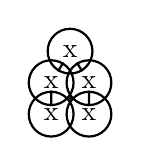
\begin{tikzpicture}[thick,scale=0.8]
   		\node at (0,0) [circle,draw] (a) {x};
       	\node at (-0.3,-0.5) [circle,draw] (b1) {x};
        \node at (0.3,-0.5) [circle,draw] (b2) {x};
        \node at (-0.3,-1) [circle,draw] (c1) {x};
        \node at (0.3,-1) [circle,draw] (c2) {x};
        \draw (a) -- (b1) -- (c1) (a) -- (b2) -- (c2) (b1) -- (c2) (b2) -- (c1);
    \end{tikzpicture} \\ 

   \hline
  \end{tabular}
\end{table}

	For the creation of the datasets used the models described in by Fussman and Heber in \textit{"Food web complexity and chaotic population dynamics"} were adopted (Fussman \& Heber, 2002). To limit the number of classes, only the eight topologies demonstrating the highest amount of chaos were used (Table 1). While evaluating these models all parameter values were kept consistent to those used by Fussman and Heber in order to ensure that the time series generated would be similarly consistent. For the convenience of the reader the general form of the differential equations describing the food web in Fig. 2 are presented:
    
\begin{multline}
	\frac{dP_i}{dt} =
    P_i\Bigg{[} 
    	r_i(1-\frac{P_i}{K_i}) - 
    	\frac{a_{P_i}^{C_1}C_1}{1 + b_{P_1}^{C_1}P_1 + b_{P_2}^{C_1}P_2 + b_{P_2}^{C_1}P_3} \\
   		-  \frac{a_{P_i}^{C_2}C_2}{1 + b_{P_1}^{C_2}P_1 + b_{P_2}^{C_2}P_2 + b_{P_2}^{C_2}P_3} \\
    	- \frac{a_{P_i}^{X}X}{1 + b_{P_1}^{X}P_1 + b_{P_2}^{X}P_2 + b_{P_3}^{X}P_3 + b_{C_1}^{X}C_1 + b_{C_2}^{X}C_2}
	\Bigg{]}, \\
    i = 1,2,3
\end{multline}

\begin{multline}
	\frac{dC_i}{dt} =
   	C_i\Bigg{[} 
    	\frac{a_{P_1}^{C_i}P_1 + a_{P_2}^{C_i}P_2 + a_{P_2}^{C_i}P_3}{1 + b_{P_1}^{C_i}P_1 + b_{P_2}^{C_i}P_2 + b_{P_2}^{C_i}P_3} \\
        - \frac{a_{C_i}^{X}X}{1 + b_{P_1}^{X}P_1 + b_{P_2}^{X}P_2 + b_{P_3}^{X}P_3 + b_{C_1}^{X}C_1 + b_{C_2}^{X}C_2} - d_{C_i}
    \Bigg{]} \\
    i = 1,2
\end{multline}

\begin{multline}
	\frac{dX}{dt} =
   		X\Bigg{[} 
        \frac{{a_{P_1}^{X}P_1 + a_{P_2}^{X}P_2 + a_{P_3}^{X}P_3 + a_{C_1}^{X}C_1 + a_{C_2}^{X}C_2}}{{1 + b_{P_1}^{X}P_1 + b_{P_2}^{X}P_2 + b_{P_3}^{X}P_3 + b_{C_1}^{X}C_1 + b_{C_2}^{X}C_2}} \\ 
        - \frac{a_X^YY}{1 + b_X^YX} - d_X
        \Bigg{]}
\end{multline}

\begin{equation}
	\frac{dY}{dt} =
    Y\Bigg{[}
    	\frac{a_X^YY}{1 + b_X^YX} - \frac{a_Y^ZZ}{1 + b_Y^ZY} - d_Y
    \Bigg{]}
\end{equation}

\begin{equation}
	\frac{dZ}{dt} =
    Z\Bigg{[}
    	\frac{a_Y^ZY}{1 + b_Y^ZY}  - d_Z
    \Bigg{]}
\end{equation}


The food web topologies and differential equations shown were found to exhibit chaotic dynamics for certain parameter settings. Figure 1 shows different visualizations of one phase space trajectory of the most chaotic network topology, the chain of length 5. The three phase space trajectories in Figure 1 have nearly identical initial conditions, and over the course of 220,000 time steps diverge showing the food chains sensitivity to initial conditions and chaotic tendencies.

\subsection{Datasets}
For the task of regression, 3 datasets were created. For these datasets, the X component of the dataset \textit{D} remained unchanged, but the labels were changed to be topologic metrics. Datasets \textit{D\textsubscript{C}},  \textit{D\textsubscript{CL}}, and  \textit{D\textsubscript{LPS}} were respectively labelled with the topologic metrics connectance, characteristic length, and links per species of the 8 different food webs. In order to compare the performance of machine learning models trained on different topologic metrics, each labelling was scaled so that it laid within a [0, 1] range. To understand why this is necessary imagine two topologic metrics for a given food web, one with value 10 and the other with value 100. If a machine learning model were to estimate the first metric at a value of 9, the second with a value of 90, the model would be 10\% off the mark for both metrics. However, measuring the error using an error function such as Mean Squared Error (MSE) would show an MSE of (10 - 9)\textsuperscript{2} = 1 for the first metric, and a value of (100 – 10)\textsuperscript{2} = 100 for the second. We eliminate this problem by normalized all labels to be in the range [0, 1]. 

For the task of classification, a total of 5 datasets were created. Of these five datasets four are subsets of the original data set, denoted \textit{D}. The relationship of these datasets to one another is shown in Figure 2. \textit{D} was created by holding all parameter values constant except for the mortality rates \textit{d\textsubscript{C\textsubscript{i}}}, \textit{d\textsubscript{Y}}, \textit{d\textsubscript{Y}}, and \textit{d\textsubscript{Z}}. The n-dimensional space of mortality rates was traversed (Table 2), evaluating the differential equations (1) through (5) 200,000 time steps for each parameter combination, and omitting the first 50,232 time steps to remove initial transient behaviour of the system. Following Fussman and Heber (Fussman \& Heber, 2002), the resulting time series of length 149769, denoted \textit{x}, was recorded only if every species in the network "survived". This was carried out by only recording time series for which all species populations were greater than the threshold value $\varepsilon$ = 10\textsuperscript{-9} at time \textit{t} = 200,000. 

\textit{D} thus has the form \textit{(\textbf{X}, \textbf{Y})}, where \textit{\textbf{X}} is a vector of time series and \textit{\textbf{Y}} is a vector of labels such that each \textit{x} $\epsilon$ \textit{\textbf{X}} was generated by evaluating equations (1) through (5) corresponding to topology \textit{y} $\epsilon$ \textit{\textbf{Y}}, where \textit{\textbf{Y}} contains the topologies in Table 1. From \textit{D}, four datasets were created. The first, \textit{D\textsubscript{N}}, is of the form \textit{(\textbf{X}\textsubscript{N}, \textbf{Y}\textsubscript{N})}, where \textit{\textbf{X}\textsubscript{N}} = \textit{\textbf{X}} and each \textit{\textbf{Y}\textsubscript{Ni}} $\epsilon$ \textit{\textbf{Y}\textsubscript{N}} is a class corresponding to the number of species in topology \textit{y} $\epsilon$ \textit{\textbf{Y}}. Since the topologies in Table 1 contain between 3 and 5 species, this means that \textit{D\textsubscript{N}} contains only 3 classes. 

Each of the three classes in \textit{D\textsubscript{N}} contain time series data generated from more than one of the topologies in Table 1. For example, the class "3" in \textit{D\textsubscript{N}}, corresponding to time series generated from topologies with 3 species, contains time series data generated from topologies A2 and A3. \textit{D\textsubscript{N}} was further partitioned into \textit{D\textsubscript{3}}, \textit{D\textsubscript{4}} and \textit{D\textsubscript{5}}, where each \textit{D\textsubscript{i}}, \textit{i} = 1, 2, 3, contains data \textit{x} $\epsilon$ \textit{\textbf{X}} generated from topology \textit{y} having \textit{i} species. 

The relationship of these datasets can be understood as trees, shown in Figure 1. \textit{D} is used to determine which of the eight topologies \textit{y} $\epsilon$ \textit{\textbf{Y}} generated a given time series \textit{x} $\epsilon$ \textit{\textbf{X}} and answers the question \textit{From which network topology was a given time series generated?} Set \textit{D\textsubscript{N}} reduces the number of classes by only distinguishing each time series by the number of species in the generating network. \textit{D\textsubscript{N}} provides answers to the question \textit{How many species are in the network from which a time series was generated?} Once \textit{D\textsubscript{N}} is used to answer this question \textit{D\textsubscript{3}}, \textit{D\textsubscript{4}} and \textit{D\textsubscript{5}} can be used to differentiate between topologies with the same number of species, ultimately providing an answer to the same question that is asked by dataset \textit{D}.

This partitioning of the \textit{D} was computationally and ecologically motivated. Computationally \textit{D\textsubscript{N}}, \textit{D\textsubscript{3}}, \textit{D\textsubscript{4}} and \textit{D\textsubscript{5}} reduce the complexity of the classification by reducing the number of classes. Inferring the generating topology only using dataset \textit{D} requires classifying the data into one of 8 classes, whereas using \textit{D\textsubscript{N}}, \textit{D\textsubscript{3}}, \textit{D\textsubscript{4}} and \textit{D\textsubscript{5}} to do the same prediction requires classifying the data into one of at most 4 classes.

In the field of ecology, the exact number of species in an environment is often known: in this case there would be no need of datasets \textit{D} or \textit{D\textsubscript{N}} and the challenge of classification would be significantly reduced. 

\begin{figure}
	\centering
	\tikzstyle{every node}=[circle, draw, fill=gray,
                        inner sep=0pt, minimum width=18pt]
    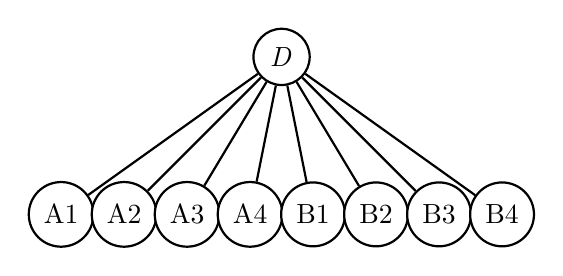
\begin{tikzpicture}[thick,scale=0.8]
   		\node at (0.0,1) [circle,draw] (a) {\textit{D}};
        \node at (-3.5,-1.5) [circle,draw,fill=white] (b) {A1};
        \node at (-2.5,-1.5) [circle,draw,fill=white] (c) {A2};
        \node at (-1.5,-1.5) [circle,draw,fill=white] (d) {A3};
        \node at (-0.5,-1.5) [circle,draw,fill=white] (e) {A4};
        \node at (0.5,-1.5) [circle,draw,fill=white] (f) {B1};
        \node at (1.5,-1.5) [circle,draw,fill=white] (g) {B2};
        \node at (2.5,-1.5) [circle,draw,fill=white] (h) {B3};
        \node at (3.5,-1.5) [circle,draw,fill=white] (i) {B4};
        \draw (a) -- (b) (a) -- (c) (a) -- (d) (a) -- (e) (a) -- (f) (a) -- (g) (a) -- (h) (a) -- (i);
    \end{tikzpicture}
\end{figure}    
    
\begin{figure}
	\centering
	\tikzstyle{every node}=[circle, draw, fill=gray,
                        inner sep=0pt, minimum width=18pt]
    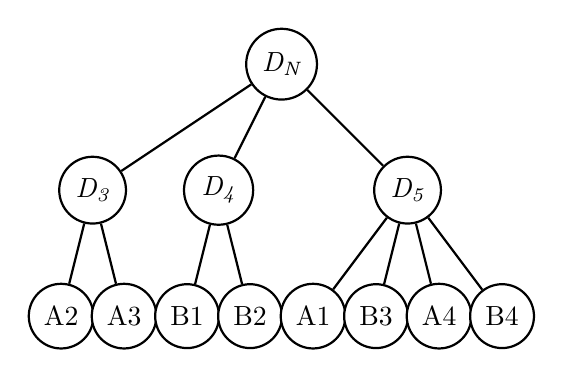
\begin{tikzpicture}[thick,scale=0.8]
    	\node at (0.0,1) [circle,draw] (a) {\textit{D\textsubscript{N}}};
        
        \node at (-3,-1) [circle,draw] (b) {\textit{D\textsubscript{3}}};
        \node at (-1,-1) [circle,draw] (c) {\textit{D\textsubscript{4}}};
        \node at (2,-1) [circle,draw] (d) {\textit{D\textsubscript{5}}};
        
        \node at (-3.5,-3) [circle,draw,fill=white] (e) {A2};
        \node at (-2.5,-3) [circle,draw,fill=white] (f) {A3};
        \node at (-1.5,-3) [circle,draw,fill=white] (g) {B1};
        \node at (-0.5,-3) [circle,draw,fill=white] (h) {B2};
        \node at (0.5,-3) [circle,draw,fill=white] (i) {A1};
        \node at (1.5,-3) [circle,draw,fill=white] (j) {B3};
        \node at (2.5,-3) [circle,draw,fill=white] (k) {A4};
        \node at (3.5,-3) [circle,draw,fill=white] (l) {B4};
        \draw (a) -- (b) (a) -- (c) (a) -- (d) (b) -- (e) (b) -- (f) (c) -- (g) (c) -- (h) (d) -- (i) (d) -- (j) (d) -- (k) (d) -- (l);
        \end{tikzpicture}
        \caption{The partitioning of data into different sets. The top tree shows data set \textit{D} as the root node, with topologies as the leaves. The bottom tree shows the relationship of \textit{D\textsubscript{3}}, \textit{D\textsubscript{4}} and \textit{D\textsubscript{5}} as subsets of \textit{D\textsubscript{N}}, with \textit{D\textsubscript{N}} being the root and topologies as the leaves}
\end{figure}


\begin{table}
\caption{Mortality Rate Parameter Space}
\setlength{\tabcolsep}{5mm} % separator between columns
\def\arraystretch{1.25} % vertical stretch factor
\centering

  \begin{tabular}{|c|c|}
	\hline
    \textbf{Parameter} & \textbf{Range} \\ \hline
    \textit{d\textsubscript{C\textsubscript{i}}}& \lbrack0.01, 1.2\rbrack \\ \hline
	\textit{d\textsubscript{X}}& \lbrack0.01, 0.42\rbrack \\ \hline
    \textit{d\textsubscript{Y}}& \lbrack0.0, 0.14\rbrack \\ \hline
    \textit{d\textsubscript{Z}}& \lbrack0.01, 0.06\rbrack \\ \hline
  \end{tabular}
\end{table}


\subsection{Classification Models}
	To classify the time series data three Machine Learning algorithms were trained and tested on the datasets described above. These algorithms, specifically a DNN, a CNN and a CNN-LSTM, were chosen because of their differences in network complexity, with the DNN being the most simple and the CNN-LSTM being the most complex, and because each possesses strengths and weaknesses in relation to certain types of data. The difference in how each algorithm performs may express some hidden trait of the ecological networks used to generate the datasets. A description of the architecture of each algorithm follows.
    
    The architecture of the DNN is a rather straightforward architecture, and was chosen to act as a pseudo baseline as DNNs are a standard first approach in most Machine Learning applications. The specific architecture featured an input layer of size 149769, followed by five hidden layers of size 50 each, with the output layer having a size equal to the number of classes in data set used. For example, if the DNN were trained and evaluated on \textit{D} the output layer would have size 8 (Fig. 3). To combat overfitting a dropout rate of 0.5 was used while training the network. 
    
    Because the size of the largest data set was still relatively small, containing only 2156 data points, a deep but skinny network architecture was favored due to a greater ability to generalize. A wide but shallow network may have memorized the data rather than computing a useful classification function. 
    
    The next most complex classification model, the CNN, was chosen as a medium complexity model to compare against the DNN. While CNNs are widely known for their use in computer vision and image classification, their ability to extract features from data autonomously has shown them to be useful in many fields (Voulodimos et al., 2018). 
    
    The CNN used utilized one-dimensional convolutions on the input to extract such features. Specifically, the architecture had an input layer of size 149769, followed by 5 hidden convolutional layers, each followed by a max pooling layer, and one fully connected layer wit a dropout rate of 0.5. This was followed by the final layer having again a size equal to the number of classes in the data set used. A complete diagram of the CNN is shown in Figure 4. 
    
    Lastly, the CNN-LSTM was chosen due to its high model complexity. LSTMs are know to excel in learning from sequential data (Graves \& Jurgen Schmidhuber, 2005), and are robust against problems of long term dependency. Because of this, the CNN-LSTM was chosen as the so-called heavy hitter of the classification algorithms. This architecture represents the combination of two preexisting architectures: it uses a series of one-dimensional convolutions which then pass the data into a LSTM layer (Fig. 5). Finally the data is passed from the LSTM cell to a fully connected layer with a dropout rate of 0.5 and to an output layer similar to those above. 
 
\begin{figure}
	\centering
    {\label{ref_label1}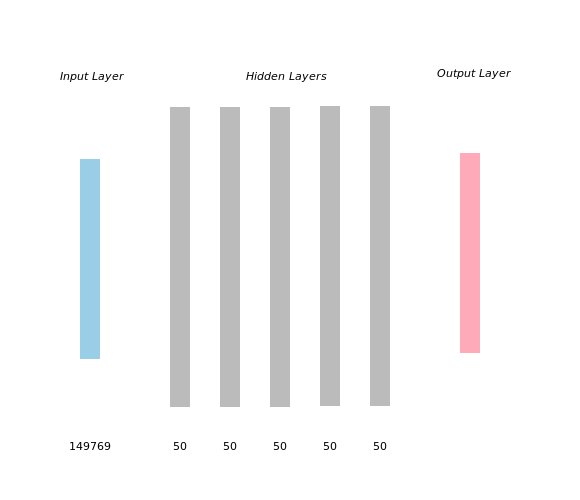
\includegraphics[width=0.5\textwidth]{dnn.png}}
    \caption{\label{ref_label_overall}The network architecture of the Deep Neural Network. The labels along the bottom represent the number of nodes in each layer. The output layer is left without a size as it will always be equal to the number of classes in the data set used to train the DNN.}
\end{figure}
 
\begin{figure}
	\centering
	{\label{ref_label1}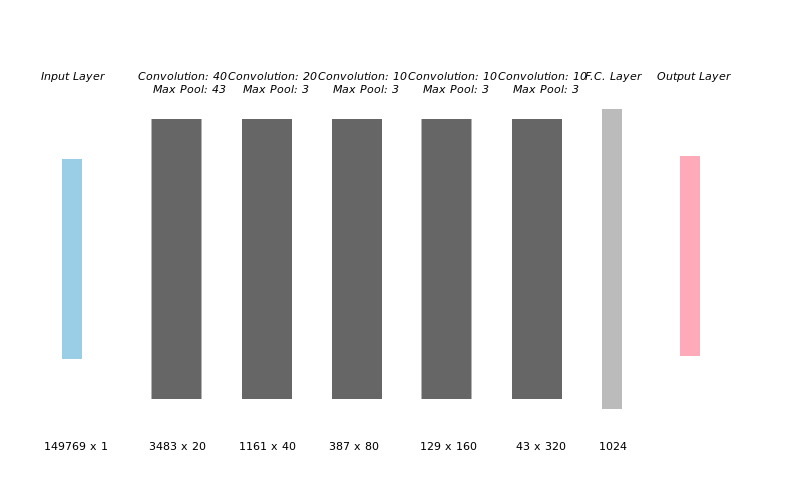
\includegraphics[width=0.5\textwidth]{cnn.png}}
    \caption{\label{ref_label_overall}The network architecture of the Convolutional Neural Network (CNN). The labels along the bottom represent the dimension of each convolutional layer or the number of nodes in a layer. The output layer is left without a size as it will always be equal to the number of classes in the data set used to train the CNN.}
\end{figure} 

\begin{figure}
	\centering
    {\label{ref_label2}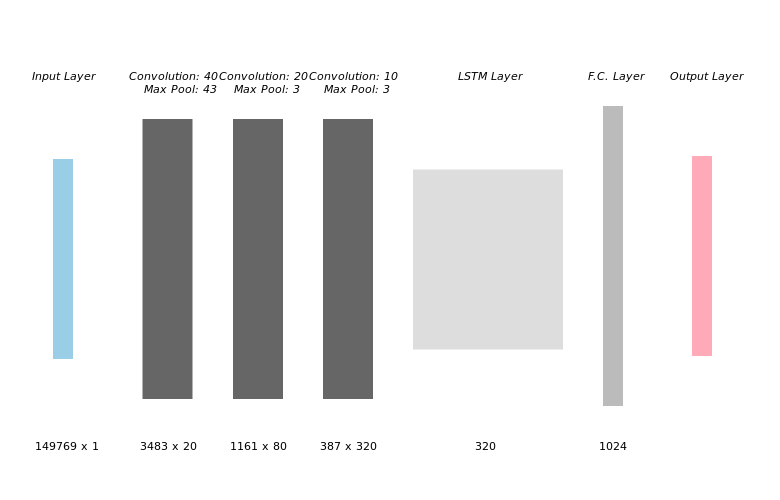
\includegraphics[width=0.5\textwidth]{cnn_lstm.png}}
    \caption{\label{ref_label_overall}The network architecture of the Convolutional Long Short Term Memory Network (CNN-LSTM). The labels along the bottom represent the dimension of each convolutional layer or the number of nodes in a layer. The output layer is left without a size as it will always be equal to the number of classes in the data set used to train the CNN-LSTM.}
\end{figure} 

%%%%%%%%%%%%%%%%%%%%%%%%%%%%%%%%%%%%%%%%%%%%%%%%%%%%%%%%%%%%%%%%%%%%%%%%%%%%%%%%
\section{METHODS}
\subsection{Dataset Creation}
	All datasets constructed using the ecological models above implemented in python. To approximate the integration of equations (1) through (5) the following form was used:
\begin{equation}x_{t+1} = x_{t} + f(x_{t})dt\end{equation}
where \textit{x\textsubscript{t}} represents the population of species \textit{x} at time \textit{t}, \textit{f($\cdot$)} is an ecological model (Equations (1) through (5)), and \textit{dt} is approximated as 0.01. 
	
    After the datasets were created, every fourth entry was withheld from training to be used in a validation set. This resulted in training and test sets that possessed identical class distributions which will be a focus of later discussion.

\subsection{Classification Models}
	The classification models used were implemented in Python, using existing TensorFlow packages for DNNs, CNNs, and LSTMs. For all the models parameters were initialized randomly and a Rectified Linear Unit (ReLu) activation function was used. For the networks containing convolutional layers same padding was used, and filters were initialized according to a random normal distribution with $\mu$ = 0 and $\sigma$ = 0.05. A learning rate of 0.001 was used for all algorithms. 
    
    During training care was taken to train all algorithms identically. All models were trained using a batch size of 50, and performance was evaluated on the withheld test set every 200 training steps. The classifiers were trained up to 2,000 training steps and the highest accuracy was recorded. The performance of the algorithms is presented in the following section. 
    
\subsection{Regression Models}
    The machine learning models for the task of regression are simply modified versions of the machine learning models for classification. For the DNN regressor, a canned tensorflow DNN regressor was used. For the CNN and CNN-LSTM the softmax function just before the output layer was removed to preserve the raw output value.  For all regressors the evaluation metric was changed from Accuracy to Mean Square Error (MSE). 

%%%%%%%%%%%%%%%%%%%%%%%%%%%%%%%%%%%%%%%%%%%%%%%%%%%%%%%%%%%%%%%%%%%%%%%%%%%%%%%%
\section{RESULTS}
	After training each algorithm and recording the results it became clear that a positive correlation between algorithm complexity and accuracy was present. For the majority of datasets the CNN-LSTM performed significantly better than the more simple classification models (Table 3).
	
    Before discussing the implications of the results, it is important to draw attention to certain patterns within the results. Firstly, it should be noted that on data set \textit{D} there is a very slight negative correlation between algorithm complexity and accuracy. Despite this, we see that the difference in accuracies on data set \textit{D} are considerably smaller than those in the other datasets. Second, one should attend to the results pertaining to data set \textit{D\textsubscript{5}} where all algorithms performed identically. Both of these patterns seem to conflict with the stronger correlation present when the algorithms were training on datasets \textit{D\textsubscript{N}}, \textit{D\textsubscript{3}} or \textit{D\textsubscript{4}} and will comprise much of the following discussion section. 

\begin{table}
\caption{Accuracy of Classification Models on datasets}
\setlength{\tabcolsep}{5mm} % separator between columns
\def\arraystretch{1.25} % vertical stretch factor
\centering

  \begin{tabular}{|c|c|c|c|}
	\hline
    & \textbf{DNN} & \textbf{CNN} & \textbf{CNN-LSTM} \\ \hline
    \textbf{\textit{D}} & \textbf{0.50} & 0.49 & 0.48 \\ \hline
    \textbf{\textit{D\textsubscript{N}}} & 0.46 & 0.60 & \textbf{0.66} \\ \hline
    \textbf{\textit{D\textsubscript{3}}} & 0.53 & 0.61 & \textbf{0.74} \\ \hline
    \textbf{\textit{D\textsubscript{4}}} & 0.77 & 0.78 & \textbf{0.84}\\ \hline
    \textbf{\textit{D\textsubscript{5}}} & 0.8 & 0.8 & 0.8 \\ \hline
  \end{tabular}
\end{table}

%%%%%%%%%%%%%%%%%%%%%%%%%%%%%%%%%%%%%%%%%%%%%%%%%%%%%%%%%%%%%%%%%%%%%%%%%%%%%%%%
\section{DISCUSSION}
	
    The results presented in the previous section are thought provoking as well as enlightening. In both the tasks of regression and classification, a trend is seen where the complexity of the model directly correlates with its performance. This will allow further research to focus efforts on models that are more successful at interpreting chaotic population data. 

    In the task of regression, we see that not all topologic metrics are created equal: it appears that the Characteristic Path Length was the ‘hardest’ metric to regress, followed by Connectance, and finally Links per Species.
    
    In this discussion, we will use modern deep learning concepts and observations about the time series data to understand the difference in performance between the models. Following that we will discuss the topologic metrics used in regression to try to understand why certain metrics seemed ‘easier’ to regress. Finally, we will use the first two discussion sections to explore the ecological relevance of these findings. It is hoped that by building a multidisciplinary understanding, a larger audience will find the results relevant and the arguments will be stronger. 

\subsection{Deep Learning}

    The performance results of the three different machine learning models are consistent with known properties of these models. In the academic and commercial realms, different types of Artificial Neural Networks (ANNs) excel at different tasks: knowing which ANN performs the best is not only useful, but can expose underlying trends in the data that the model is using. Similarly, observations about the data can help inform which ANN(s) may be best for the task at hand. 

    For example, CNNs are known to be shift invariant, meaning they can learn features in data that are shifted an arbitrary amount in each sample (Norouzi et al., 2009). CNNs excel at classifying images in which the subject (i.e. a car) may be shifted, rotated, or otherwise changed. A CNN typically overcomes these shifts by extracting common features of the data and using them to make a more informed decision. To classify an image of a car, the CNN may extract high level features like a tire, or a mirror and use the collection of features present to determine what the image is: if it has four wheels and two mirrors it is probably a car. 

    \begin{figure}
    {\label{ref_label1}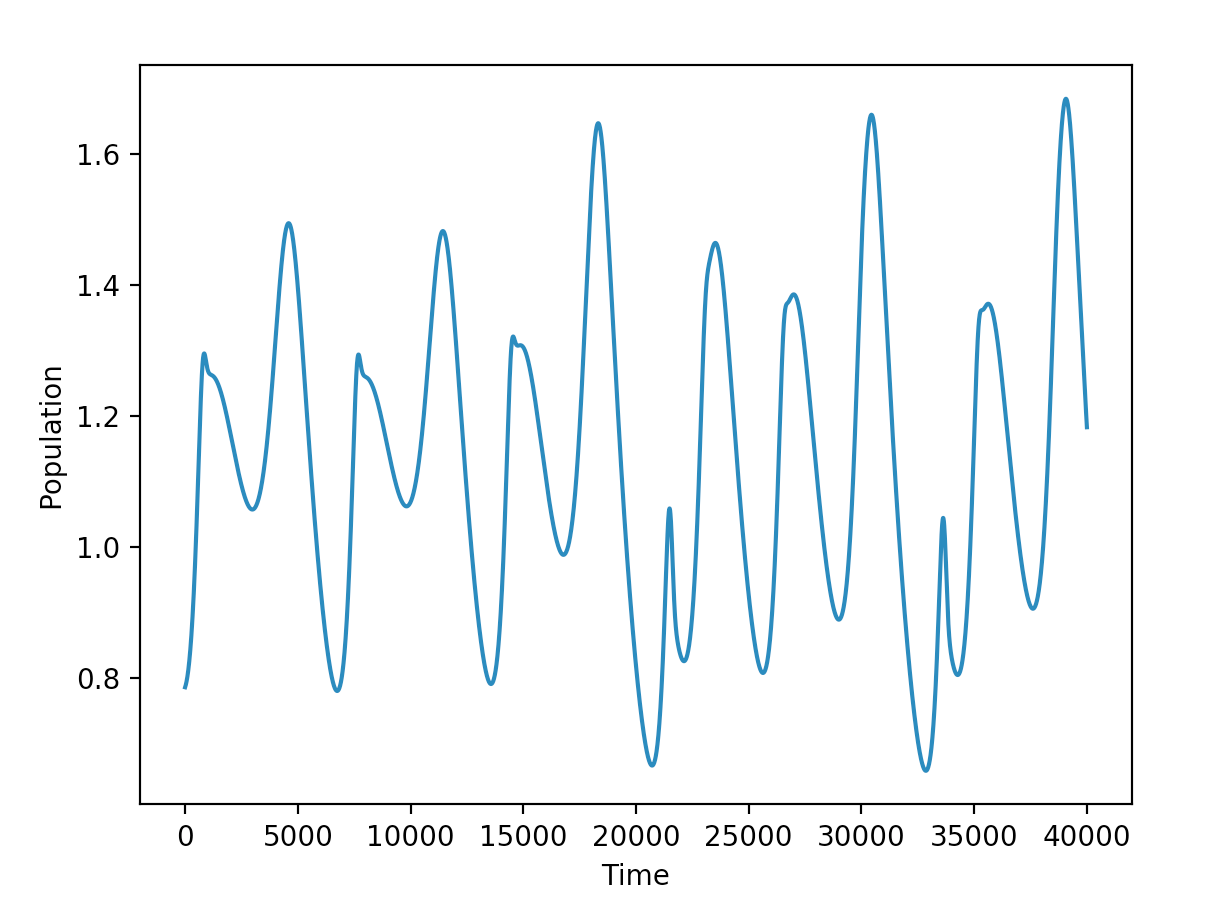
\includegraphics[width=0.5\textwidth]{dataspikes.png}}
        \caption{\label{ref_label_overall}Time series showing spikes at irregular intervals and magnitudes. Notice that even spikes of similar shape return in a slightly altered form. This type of series may be best understood by networks containing LSTM cells.}
    \end{figure} 
    \begin{table}
        \caption{Class Distribution of datasets}
        \setlength{\tabcolsep}{5mm} % separator between columns
        \def\arraystretch{1.25} % vertical stretch factor
        \centering
        \begin{tabular}{|c|c|c|c|c|c|}
	        \hline
            & \textbf{\textit{D}} &  \textbf{\textit{D\textsubscript{N}}} &      \textbf{\textit{D\textsubscript{3}}} &  \textbf{\textit{D\textsubscript{4}}} &      \textbf{\textit{D\textsubscript{5}}}\\ \hline
            \textbf{0} & 0.34 & 0.44 & 0.45 & 0.24 & 0.80\\ \hline
            \textbf{1} & 0.34 & 0.45 & 0.55 & 0.76 & 0.04\\ \hline
            \textbf{2} & 0.05 & 0.11 &  &  & 0.02\\ \hline
            \textbf{3} & 0.06 &  &  &  & 0.14\\ \hline
            \textbf{4} & 0.11 &  &  &  & \\ \hline
            \textbf{5} & 0.03 &  &  &  & \\ \hline
            \textbf{6} & 0.02 &  &  &  & \\ \hline
            \textbf{7} & 0.05 &  &  &  & \\ \hline
        \end{tabular}
    \end{table}

    If one see’s that a CNN is outperforming a DNN it is logical to ask “what aspects of the data are easier for the CNN?”. To answer this question, it is important to look at the data the CNN and DNN were trained and evaluated on.  Figure 6 shows the time series of one species’ population generated from the ecological models explained above. At first glance, this data appears to be somewhat cyclic, with similarly shaped spikes occurring at regular intervals. However, the astute observer will notice that the peak of each spike is slightly different and that the spacing between spikes is not uniform. There are two theories for why the CNN outperformed the DNN that relate the data used and the known properties of the CNN. Firstly, one can imagine that the CNN is learning features that correspond to unique spike shapes, disregarding the frequency at which these spikes appear, and using this distinct spike shape to classify time series. Second, the small irregularities in spike shape and location can be understood as a shift applied to some original spike form. Both theories provide an explanation for why the CNN would outperform the DNN using the data supplied to it. 

    Likewise, the addition of an LSTM cell to a CNN to create the LSTM-CNN was inspired by known properties of LSTM networks. Because the CNN-LSTM is comprised partially of a CNN any change in performance cause by adding an LSTM cell would logically be caused by that LSTM cell. We see that the CNN-LSTM outperforms the CNN: the logical conclusion is that the LSTM cell helped the CNN. Again, the question “what aspects of the data are easier for the CNN-LSTM?” should be asked. 
    
    The increased performance in the CNN-LSTM can again be explained by known properties of LSTM cells and observations about the data. LSTMs are known to excel at problems that feature long term dependencies, or events which occur at unknown intervals (Lipton & Berkowitz, 2015). Because of this, one can intuit that random shifts of similarly shaped spikes in a time series may cause a CNN to underperform in comparison to a CNN-LSTM. Since the CNN-LSTM is comprised of convolutional layers followed by an LSTM cell one can think of the classifier as first extracting features (spike shapes) using convolutions, then addressing the random spacing between them by passing the resulting features to an LSTM cell. This understanding aligns with the theory that the CNN layers learn time series features in the form of spike shapes. The CNN learns spike shapes better than the DNN, but gets somewhat confused by the random intervals between them and therefor is aided by the addition of an LSTM cell. These observations about the data and the properties of different machine learning models provide an explanation for the increased accuracy in the CNN and CNN- LSTM. 

    In the task of classification, special attention should be paid to the datasets \textit{D} and \textit{D\textsubscript{5}} which do not show the more complex classifiers performing better. Unsurprisingly, \textit{D} remained the least classifiable of the datasets. This could be explained by the fact that this set contained the greatest number of classes. Considering Table 3, it is seen that all classifiers perform significantly better than a baseline estimator, but reach approximately the same accuracy when trained and evaluated on dataset \textit{D}. Because of the minimal difference between performances, it is hypothesized that \textit{D} is not completely classifiable. This apparent similarity between chaotic dynamics of different topologies may be explained by looking strictly at the topologies themselves. Consider topology A1, the five-species chain. Topologies B1 (the four-species chain), and A2 (the three species chain) are sub-graphs of A1: it may be possible that the chaotic dynamics created from A1 may also be created from B1 or A2. If this were true then those dynamics stem from multiple topologies would be unclassifiable. Similarly, one can see that topology A2 is a sub-graph of every other topology, potentially contributing to the classifiability of the data set. 

    The data set \textit{D\textsubscript{5}} presents a different phenomenon. The accuracy of each algorithm was identical; furthermore, the accuracy of each algorithm was exactly that of a baseline classifier. Essentially,  each algorithm simply learned to guess the most common class in the data set \textit{D\textsubscript{5}}. Table 4 shows the class distribution of each data set. From this one can see that the most common class in \textit{D\textsubscript{5}} comprised 80\% of the data points. While this may be underwhelming in regards to the learning capabilities of the algorithms, it may be important in regards to the ecological models. 

    Fussman and Heber showed that topology A1 possessed the highest percentage of chaotic parameters of all topologies they tested. Unsurprisingly, the class representing 80\% of data set \textit{D\textsubscript{5}} was none other than topology A1. The non-uniformity in the distribution of classes in \textit{D\textsubscript{5}} matches the findings of Fussman and Heber and may be more useful than any fancy Machine Learning Algorithm. Because a 5-species chain is so chaotic, it may be useful to know that chaotic dynamics found in a five-species system most likely come from a chain of five species. Furthermore, the inability of all algorithms to classify chaotic time series generated from topologies of five species with more success than a baseline classifier may indicate that the time series themselves are nearly identical. 
    
    Datasets \textit{D} and \textit{D\textsubscript{5}} are particularly helpful in defining future research in the topic of chaotic time series classification. Future work may include creating an analogue to \textit{D\textsubscript{5}} which features a more even class distribution, or removing the topology A1 from the data set entirely to distinguish topologies of similar levels of chaos. 

    To test the similarity of time series generated by topologies, the visualization of attractors from these topologies would be extremely helpful. If attractors look similar it would provide evidence that \textit{D} is indeed impossible to classify perfectly. 
    
    Lastly, it is recommended that research be conducted using classification algorithms which are adept at learning from chaotic time series data. Further research into architectures using LSTM cells seems to be a logical direction to start in. Architectures such as Liquid State Machines (LSMs) or Echo State Networks (ESNs) have been shown to excel at predicting and classifying chaotic data and could be the focus of further experimentation (Li et al., 2012). 

\subsection{Topologic Metrics}

    Not only was a trend in machine learning models performance shown, but a trend in which metrics resulted in the best performance was also seen. As stated above, all models performed the poorest (i.e. had the highest loss values) when regressing in terms of the Characteristic Path Length of a given topology. The results of the models on the other two metrics, the Connectance and Links per Species, were much more similar but Links per Species had the lowest loss in most scenarios. 

    One way to gain insight into the usability of the three metrics is to simply visualize them. Figure 7 shows that even after normalization to the 0-1 range, the different metrics have different qualities. The most notable feature of the regression metrics is the ‘evenness’ of each metric. The Characteristic Path Length is the less ‘even’ of all the metrics. This ‘unevenness’ of the Characteristic Path Length may be one reason why the metric is harder to regress. To understand this, imagine that you are tasked with guessing the Characteristic Path Length associated with a time series. It seems risky to guess a value higher than 0.4 since the majority (6 of 8) of labels fall within 0 to 0.4. 

    To calculate evenness of a system more concretely one can use the interquartile range (IQR). The IQR of the Characteristic Path Lengths of the topologies is 0.35, the IQR of the Connectances is 0.65 and is 0.59 for the Links per Species’ values. These values partially explain the difference in performance when regressing different topologic values. The lower IQR  for the Characteristic Path Length confirms that those values are much more unevenly grouped, and the similar IQR values for Connectance and Links per Species align with the roughly similar loss trends when training and evaluating on Connectance and Links per Species. 
    
    However, following this logic one would expect to see higher performance when training and evaluating on Connectance than when training and evaluating on Links per Species, which is contrary to the results presented. It may be that groups or unevenness are not intrinsically bad, but that there are better groupings than others. Looking at how each metric groups each corresponding topology along the number line may offer a hint as to why Links per Species proved to be a better metric to use. The Characteristic Path Length groups the topologies B2, B3, A4, A2 and B4 closely together. The Connectance has less distinct groups, but groups the three chain topologies A1, B2 and A2 together, as well as the topologies B2 and B3. The Links per Species similarly groups the chain topologies together, but groups them more closely together than Connectance. It also groups together topologies B2 and B4. 
    
\begin{figure}
    \centering
        
    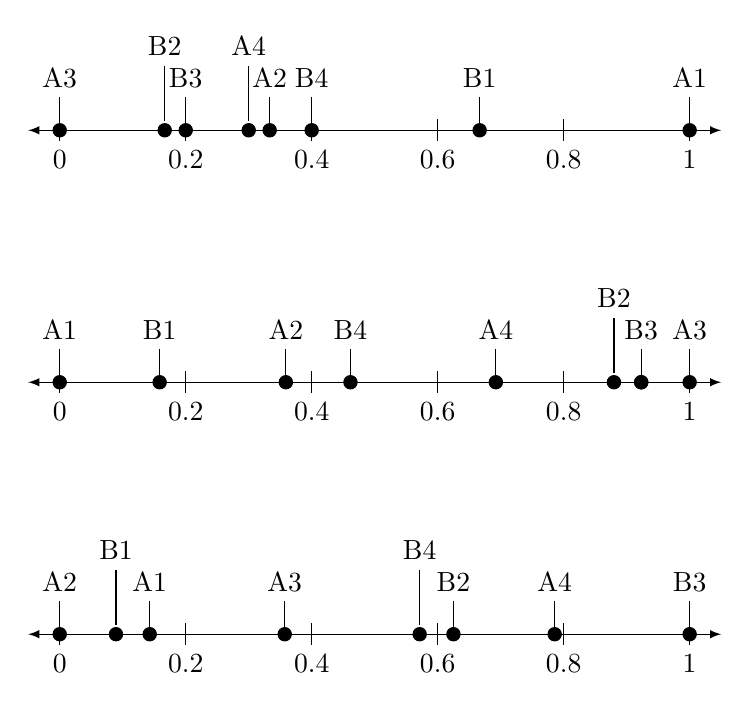
\begin{tikzpicture}[scale=8]
        \path [draw=black, fill=black] (0,0.4) circle (0.3pt);
        \draw[shift={(0,0.4)},color=black] (0pt,0pt) -- (0pt,1.5pt) node[above]
        {A3};
        \path [draw=black, fill=black] (0.16666,0.4) circle (0.3pt);
        \draw[shift={(0.16666,0.45)},color=black] (0pt,-1pt) -- (0pt,1.5pt) node[above]
        {B2};
        \path [draw=black, fill=black] (0.2,0.4) circle (0.3pt);
        \draw[shift={(0.2,0.4)},color=black] (0pt,0pt) -- (0pt,1.5pt) node[above]
        {B3};
        \path [draw=black, fill=black] (0.3,0.4) circle (0.3pt);
        \draw[shift={(0.3,0.45)},color=black] (0pt,-1pt) -- (0pt,1.5pt) node[above]
        {A4};
        \path [draw=black, fill=black] (0.33333,0.4) circle (0.3pt);
        \draw[shift={(0.33333,0.4)},color=black] (0pt,0pt) -- (0pt,1.5pt) node[above]
        {A2};
        \path [draw=black, fill=black] (0.4,0.4) circle (0.3pt);
        \draw[shift={(0.4,0.4)},color=black] (0pt,0pt) -- (0pt,1.5pt) node[above]
        {B4};
        \path [draw=black, fill=black] (0.66666,0.4) circle (0.3pt);
        \draw[shift={(0.66666,0.4)},color=black] (0pt,0pt) -- (0pt,1.5pt) node[above]
        {B1};
        \path [draw=black, fill=black] (1,0.4) circle (0.3pt);
        \draw[shift={(1,0.4)},color=black] (0pt,0pt) -- (0pt,1.5pt) node[above]
        {A1};
        \draw[latex-latex] (-0.05,0.4) -- (1.05,0.4) ;
        \foreach \x in  {0, 0.2, 0.4, 0.6, 0.8, 1}
        \draw[shift={(\x,0.4)},color=black] (0pt,0.5pt) -- (0pt,-0.5pt);
        \foreach \x in {0, 0.2, 0.4, 0.6, 0.8, 1}
        \draw[shift={(\x,0.4)},color=black] (0pt,0pt) -- (0pt,-0.5pt) node[below] 
        {$\x$};
        
        \path [draw=black, fill=black] (0,0) circle (0.3pt);
        \draw[shift={(0,0)},color=black] (0pt,0pt) -- (0pt,1.5pt) node[above] 
        {A1};
        \path [draw=black, fill=black] (0.158656897248,0) circle (0.3pt);
        \draw[shift={(0.158656897248,0)},color=black] (0pt,0pt) -- (0pt,1.5pt) node[above]
        {B1};
        \path [draw=black, fill=black] (0.358968441701,0) circle (0.3pt);
        \draw[shift={(0.358968441701,0)},color=black] (0pt,0pt) -- (0pt,1.5pt) node[above]
        {A2};
        \path [draw=black, fill=black] (0.461547337449,0) circle (0.3pt);
        \draw[shift={(0.461547337449,0)},color=black] (0pt,0pt) -- (0pt,1.5pt) node[above]
        {B4};
        \path [draw=black, fill=black] (0.692321006173,0) circle (0.3pt);
        \draw[shift={(0.692321006173,0)},color=black] (0pt,0pt) -- (0pt,1.5pt) node[above]
        {A4};
        \path [draw=black, fill=black] (0.879824612012,0) circle (0.3pt);
        \draw[shift={(0.879824612012,0.05)},color=black] (0pt,-1pt) -- (0pt,1.5pt) node[above]
        {B2};
        \path [draw=black, fill=black] (0.923094674898,0) circle (0.3pt);
        \draw[shift={(0.923094674898,0)},color=black] (0pt,0pt) -- (0pt,1.5pt) node[above]
        {B3};
        \path [draw=black, fill=black] (1,0) circle (0.3pt);
        \path [draw=black, fill=black] (0.923094674898,0) circle (0.3pt);
        \draw[shift={(1,0)},color=black] (0pt,0pt) -- (0pt,1.5pt) node[above]
        {A3};
        \draw[latex-latex] (-0.05,0) -- (1.05,0) ;
        \foreach \x in  {0, 0.2, 0.4, 0.6, 0.8, 1}
        \draw[shift={(\x,0)},color=black] (0pt,0.5pt) -- (0pt,-0.5pt);
        \foreach \x in {0, 0.2, 0.4, 0.6, 0.8, 1}
        \draw[shift={(\x,0)},color=black] (0pt,0pt) -- (0pt,-0.5pt) node[below] 
        {$\x$};
        
        \path [draw=black, fill=black] (0,-0.4) circle (0.3pt);
        \draw[shift={(0,-0.4)},color=black] (0pt,0pt) -- (0pt,1.5pt) node[above] 
        {A2};
        \path [draw=black, fill=black] (0.0892922193413,-0.4) circle (0.3pt);
        \draw[shift={(0.0892922193413,-0.35)},color=black] (0pt,-1pt) -- (0pt,1.5pt) node[above] 
        {B1};
        \path [draw=black, fill=black] (0.142863265262,-0.4) circle (0.3pt);
        \draw[shift={(0.142863265262,-0.4)},color=black] (0pt,0pt) -- (0pt,1.5pt) node[above] 
        {A1};
        \path [draw=black, fill=black] (0.357147448947,-0.4) circle (0.3pt);
        \draw[shift={(0.357147448947,-0.4)},color=black] (0pt,0pt) -- (0pt,1.5pt) node[above] 
        {A3};
        \path [draw=black, fill=black] (0.571431632631,-0.4) circle (0.3pt);
        \draw[shift={(0.571431632631,-0.35)},color=black] (0pt,-1pt) -- (0pt,1.5pt) node[above] 
        {B4};
        \path [draw=black, fill=black] (0.625002678552,-0.4) circle (0.3pt);
        \draw[shift={(0.625002678552,-0.4)},color=black] (0pt,0pt) -- (0pt,1.5pt) node[above] 
        {B2};
        \path [draw=black, fill=black] (0.785715816316,-0.4) circle (0.3pt);
        \draw[shift={(0.785715816316,-0.4)},color=black] (0pt,0pt) -- (0pt,1.5pt) node[above] 
        {A4};
        \path [draw=black, fill=black] (1,-0.4) circle (0.3pt);
        \draw[shift={(1,-0.4)},color=black] (0pt,0pt) -- (0pt,1.5pt) node[above] 
        {B3};
        \draw[latex-latex] (-0.05,-0.4) -- (1.05,-0.4) ;
        \foreach \x in  {0, 0.2, 0.4, 0.6, 0.8, 1}
        \draw[shift={(\x,-0.4)},color=black] (0pt,0.5pt) -- (0pt,-0.5pt);
        \foreach \x in {0, 0.2, 0.4, 0.6, 0.8, 1}
        \draw[shift={(\x,-0.4)},color=black] (0pt,0pt) -- (0pt,-0.5pt) node[below] 
        {$\x$};
        
    \end{tikzpicture}
    
    \caption{The values of topologic metrics and their associated topologies plotted on a number line. The top numberline shows the values for the Characteristic Path Length, the middle number line the values for Connectance and the bottom number line the values for Links per Species.}

\end{figure}

    The facts that certain topologies a) result in different performances and b) group the topologies differently implies that certain groupings of topologies are easier to regress than others. Furthermore, this implies that the groupings of topologies that are ‘easier’ to regress group the topologies such that each group contains topologies that generate time series that are similar to each other. For example, the fact that the ‘easier’ metrics Connectance and Links per Species metrics grouped the chain topologies together implies that the time series generated by these chains are similar – if the regressors saw a time series that corresponded to a chain topology, it was regressed into the area of the number line reserved for chain topologies. This contrasts a regressor trained and evaluated using the Characteristic Path Length which, finding a time series corresponding to a chain topology, would not have a convenient region to regress into. 

    This realization is interesting in the fact that it also implies that certain topologic metrics may reflect the generating properties of a system better than others. As previously mentioned, future work in comparing similarities in time series generated by these topologies would be immensely helpful.

\subsection{Ecologic Relevance}

    TODO
    
%\addtolength{\textheight}{-12cm}   % This command serves to balance the column lengths
                                  % on the last page of the document manually. It shortens
                                  % the textheight of the last page by a suitable amount.
                                  % This command does not take effect until the next page
                                  % so it should come on the page before the last. Make
                                  % sure that you do not shorten the textheight too much.

%%%%%%%%%%%%%%%%%%%%%%%%%%%%%%%%%%%%%%%%%%%%%%%%%%%%%%%%%%%%%%%%%%%%%%%%%%%%%%%%
\section{CONCLUSIONS}
	The presence of chaos in the natural and unnatural world has sparked the interest of many of the greatest minds of our time. Its seemingly random, yet deterministic nature has been found throughout our world and others and has been shown to help explain many difficult phenomena. In the natural world the presence of chaos in ecological systems, particular in their cycles of populations, has allowed for further in depth analysis of the world around us. 

	The precise aspect of chaos that draws many to it makes it puzzling to those who ponder it. It's difficulty to characterize and predict has challenged many researchers. Using different Machine Learning algorithms, this report has strove to gain an insight into chaos, showing that for the specific task of topological inference in ecologic networks, complex models such as a CNN-LSTM can better capture the essence of the data. This finding enlightens future researchers by giving a sturdier understanding of the characteristics and tools needed to analyze chaotic populations. 
    
    It is suggested that future research focus on the development of (1) a higher quality dataset with more even class distributions, and (2) classification models more capable of understanding the data. Also of interest would be (3) the determination of whether or not chaotic time series produced by the models used above are indeed classifiable. 
    
%%%%%%%%%%%%%%%%%%%%%%%%%%%%%%%%%%%%%%%%%%%%%%%%%%%%%%%%%%%%%%%%%%%%%%%%%%%%%%%%
\section{ACKNOWLEDGMENTS}
		Many thanks are owed to those individuals who took time to aid in the completion of this report. Frederic Guichard, the supervisor of this study, provided endless insight into the world of chaos and dynamical systems which I had not had any previous training in. Professor Guichard aided in narrowing the scope of the project to a manageable size, and pointed research in a helpful direction when roadblocks were met. He encouraged me to pursue publication and has been an academic inspiration even after my time at University has ended. I would like to thank also, and perhaps strangely, my trumpet teacher Russel DeVuyst for leading by example and teaching lessons that could be carried far outside of the practice room, showing that age does not need to diminish curiosity and enthusiasm, and for understanding that my interests spanned many disciplines. To my family are owed the greatest thanks, for their support and love, for their ability to listen to rants filled with mathematical terminology and endless requests to look at strange attractors. Lastly, I would like to thank 5b's Bakery in Concrete, Washington for providing me with a space to camp out for many hours on end to complete the report, and for their endless coffee. 

%%%%%%%%%%%%%%%%%%%%%%%%%%%%%%%%%%%%%%%%%%%%%%%%%%%%%%%%%%%%%%%%%%%%%%%%%%%%%%%%
\begin{thebibliography}{99}

\bibitem{c1}Decai Li, Min Han and Jun Wang. “Chaotic Time Series Prediction Based on a Novel Robust Echo State Network.” IEEE Transactions on Neural Networks and Learning Systems 23: 787-799. (2012).

\bibitem{c2} Thomas G. Dietterich. "Machine Learning for Sequential Data: A Review". Structural, Syntactic, and Statistical Pattern Recognition, Lecture Notes in Computer Science, vol 2396. (2002).

\bibitem{c3} Edward N Lorenz. "The Essence of Chaos". University of Washington Press. (1993).

\bibitem{c4} Gregor F. Fussmann and Gerd Heber. “Food web complexity and chaotic population dynamics.” (2002).

\bibitem{c5} Luis J. Gilarranz, Alan Hastings, and Jordi Bascompte. "Inferring topology from dynamics in spatial networks". Theor Ecol 8: 15. https://doi.org/10.1007/s12080-014-0231-y. (2015).

\bibitem{c6} Alex Graves and Jurgen Schmidhuber. "Framewise phoneme classification with bidirectional LSTM and other neural network architectures". Neural Networks, 18:602–610. (2005).

\bibitem{c7} Aaron Klebanoff and Alan Hastings. "Chaos in one-predator, two-prey models: general results from bifurcation theory." A. J. Math. Biol. 32: 427. https://doi.org/10.1007/BF00160167. (1994).

\bibitem{c8}Aaron Klebanoff and Alan Hastings (1994). "Chaos in three species food chains". J. Math. Biol. 32, 427–451. (1994).

\bibitem{c9} Jacques Maquet and Christophe Letellier. "Global models from the Canadian lynx cycles as a direct evidence for chaos in real ecosystems".  L.A. J. Math. Biol. 55: 21. https://doi.org/10.1007/s00285-007-0075-9. (2007)

\bibitem{c10} Marc Barthelemy, Jean-Pierre Nadal, and Henri Berestycki. PNAS 107 (17) 7629-7634;https://doi.org/10.1073/pnas.0910259107. 

\bibitem{c12} Mohammad Norouzi, Mani Ranjbar, and Greg Mori. "Stacks of convolutional Restricted Boltzmann Machines for shift-invariant feature learning". IEEE Conference on Computer Vision and Pattern Recognition. (2009).

\bibitem{c12} Paola Vera-Licona and Reinhard Laubenbacher. "Inference of ecological interaction networks". Annales Botanici Fennici, 45: 459-464. (2008).

\bibitem{c13} Athanasios Voulodimos, Nikolaos Doulamis, Anastasios Doulamis, and Eftychios Protopapadakis, “Deep Learning for Computer Vision: A Brief Review". Computational Intelligence and Neuroscience, vol. 2018, Article ID 7068349. https://doi.org/10.1155/2018/7068349. (2018).

\bibitem{c14} William M. Schaffer and Mark Kot. "Do Strange Attractors Govern Ecological Systems?". BioScience, Volume 35, Issue 6, 342–350, https://doi.org/10.2307/1309902. (1985).

\bibitem{c15} Zachary C. Lipton, John Berkowitz, and Charles Elkan. "A critical review of recurrent neural networks for sequence learning". arXiv preprint arXiv:1506.00019. (2015).
\end{thebibliography}

\end{document}